\documentclass[a4paper,12pt,twoside,onecolumn,openright,final,oldfontcommands]{memoir}
\usepackage{lmodern}
\usepackage{amssymb,amsmath}
\usepackage{ifxetex,ifluatex}
\usepackage{fixltx2e} % provides \textsubscript
\usepackage[T1]{fontenc}
\usepackage[utf8]{inputenc}

% use upquote if available, for straight quotes in verbatim environments
\IfFileExists{upquote.sty}{\usepackage{upquote}}{}
% use microtype if available
\IfFileExists{microtype.sty}{%
\usepackage{microtype}
\UseMicrotypeSet[protrusion]{basicmath} % disable protrusion for tt fonts
}{}
\usepackage[unicode=true]{hyperref}
\hypersetup{
            pdftitle={From the mechanistic modeling of signaling pathways in cancer to the interpretation of models and their contributions: clinical applications and statistical evaluation},
            pdfborder={0 0 0},
            breaklinks=true}
\urlstyle{same}  % don't use monospace font for urls
\usepackage{natbib}
\bibliographystyle{plainnat}
\usepackage{longtable,booktabs}
\usepackage{graphicx,grffile}
\makeatletter
\def\maxwidth{\ifdim\Gin@nat@width>\linewidth\linewidth\else\Gin@nat@width\fi}
\def\maxheight{\ifdim\Gin@nat@height>\textheight\textheight\else\Gin@nat@height\fi}
\makeatother
% Scale images if necessary, so that they will not overflow the page
% margins by default, and it is still possible to overwrite the defaults
% using explicit options in \includegraphics[width, height, ...]{}
\setkeys{Gin}{width=\maxwidth,height=\maxheight,keepaspectratio}
\IfFileExists{parskip.sty}{%
\usepackage{parskip}
}{% else
\setlength{\parindent}{0pt}
\setlength{\parskip}{6pt plus 2pt minus 1pt}
}
\setlength{\emergencystretch}{3em}  % prevent overfull lines
\providecommand{\tightlist}{%
  \setlength{\itemsep}{0pt}\setlength{\parskip}{0pt}}
\setcounter{secnumdepth}{5}
% Redefines (sub)paragraphs to behave more like sections
\ifx\paragraph\undefined\else
\let\oldparagraph\paragraph
\renewcommand{\paragraph}[1]{\oldparagraph{#1}\mbox{}}
\fi
\ifx\subparagraph\undefined\else
\let\oldsubparagraph\subparagraph
\renewcommand{\subparagraph}[1]{\oldsubparagraph{#1}\mbox{}}
\fi
%%%%%%%%%%%%%%%%%%%%%%%%%%%%%%%%%%%%%%%%%%%%%%%%%%%%%%%%%%%%%
%Start preamble
%%%%%%%%%%%%%%%%%%%%%%%%%%%%%%%%%%%%%%%%%%%%%%%%%%%%%%%%%%%%%

\usepackage{booktabs}
\usepackage{amsthm}
\usepackage{./cover/psl-cover} % specifies the path to the cover page template
%\usepackage{psl-cover} % specifies the path to the cover page template

%\makeatletter
%\def\thm@space@setup{%
%  \thm@preskip=8pt plus 2pt minus 4pt
%  \thm@postskip=\thm@preskip
%}
%\makeatother


%%%%%%%%%%%%%%%%%%%%%%%%%%%%%%%%%%%%%%%%%%%%%%%%%%%%%%%%%%%%%
% Add a lettrine to the very first character of the content %
%%%%%%%%%%%%%%%%%%%%%%%%%%%%%%%%%%%%%%%%%%%%%%%%%%%%%%%%%%%%%

\usepackage{lettrine} % supports various dropped capitals styles

\newcommand{\initial}[1]{
	\lettrine[lines=3,lhang=0.33,nindent=0em]{
		\color{gray}
     		{\textsc{#1}}}{}}
     		

%%%%%%%%%%%%%%%%%%%%%%%%%%%%%%%%%%%%%%%%%%%%%%%%%%%%%%%%%%%%%
% Links box
%%%%%%%%%%%%%%%%%%%%%%%%%%%%%%%%%%%%%%%%%%%%%%%%%%%%%%%%%%%%%
\usepackage{hyperref}
\hypersetup{
    colorlinks=true,
    linkcolor=blue,
    filecolor=blue,      
    urlcolor=blue,
    citecolor=blue
}

%%%%%%%%%%%%%%%%%%%%%%%%%%%%%%%%%%%%%%%%%%%%%%%%%%%%%%%%%%%%%
% Text box
%%%%%%%%%%%%%%%%%%%%%%%%%%%%%%%%%%%%%%%%%%%%%%%%%%%%%%%%%%%%%
\usepackage{xcolor}
\usepackage{tcolorbox}
\newtcolorbox{summarybox}{
  colback=lightgray,
  colframe=teal,
  coltext=black,
  boxsep=5pt,
  arc=4pt}
     		
%%%%%%%%%%%%%%%%%%%%%%%%
% Insert an empty page %
%%%%%%%%%%%%%%%%%%%%%%%%

\usepackage{afterpage} % executes command after the next page break

\newcommand\blankpage{%
    \null
    \thispagestyle{empty}%
    % \addtocounter{page}{-1}% % uncomment to increase page counter
    \newpage
    }

\newcommand{\clearemptydoublepage}{\newpage{\thispagestyle{empty}\cleardoublepage}}

%%%%%%%%%%%%%%%%%%
% Epigraph style %
%%%%%%%%%%%%%%%%%%

\usepackage{epigraph} % provides commands to assist in the typesetting of a single epigraph

\setlength\epigraphwidth{1\textwidth}
\setlength\epigraphrule{0pt} % no line between
\setlength\beforeepigraphskip{1\baselineskip} % space before and after epigraph
\setlength\afterepigraphskip{2\baselineskip}
\renewcommand*{\textflush}{flushright}
\renewcommand*{\epigraphsize}{\normalsize\itshape}

%%%%%%%%%%%%%%%%%%%%%%%%
% Formatting
%%%%%%%%%%%%%%%%%%%%

\usepackage{calc} % simple arithmetics in latex commands
\usepackage{soul} % hyphenation for letterspacing, underlining, etc.

\makeatletter
\newlength\dlf@normtxtw
\setlength\dlf@normtxtw{\textwidth}
\newsavebox{\feline@chapter}
\newcommand\feline@chapter@marker[1][4cm]{%
	\sbox\feline@chapter{%
		\resizebox{!}{#1}{\fboxsep=1pt%
			\colorbox{gray}{\color{white}\thechapter}%
		}}%
		\rotatebox{90}{%
			\resizebox{%
				\heightof{\usebox{\feline@chapter}}+\depthof{\usebox{\feline@chapter}}}%
			{!}{\scshape\so\@chapapp}}\quad%
		\raisebox{\depthof{\usebox{\feline@chapter}}}{\usebox{\feline@chapter}}%
}

\newcommand\feline@chm[1][4cm]{%
	\sbox\feline@chapter{\feline@chapter@marker[#1]}%
	\makebox[0pt][c]{% aka \rlap
		\makebox[1cm][r]{\usebox\feline@chapter}%
	}}

\makechapterstyle{daleifmodif}{
\renewcommand\chapnamefont{\normalfont\Large\scshape\raggedleft\so}
\renewcommand\chaptitlefont{\normalfont\Large\bfseries\scshape}
\renewcommand\chapternamenum{} \renewcommand\printchaptername{}
\renewcommand\printchapternum{\null\hfill\feline@chm[2.5cm]\par}
\renewcommand\afterchapternum{\par\vskip\midchapskip}
\renewcommand\printchaptertitle[1]{\color{gray}\chaptitlefont\raggedleft
  \renewcommand\chaptername{Chapter}
  ##1\par}
}

\makeatother
\chapterstyle{daleifmodif}

% The pages should be numbered consecutively at the bottom centre of the page
\makepagestyle{myvf}
\makeoddfoot{myvf}{}{\thepage}{}
\makeevenfoot{myvf}{}{\thepage}{}
\makeheadrule{myvf}{\textwidth}{\normalrulethickness}
\makeevenhead{myvf}{\small\textsc{\leftmark}}{}{}
\makeoddhead{myvf}{}{}{\small\textsc{\rightmark}}
\pagestyle{myvf}


%%%%%%%%%%%%%%%%%%%%%%%%%%%%%%%%%%%%%%%%%%%%%%%%%%%%%%%%%%%%%
% Define cover page settings
%%%%%%%%%%%%%%%%%%%%%%%%%%%%%%%%%%%%%%%%%%%%%%%%%%%%%%%%%%%%%

\title{My title}

\author{Jonas BEAL}

\institute{l'Institut Curie}
\doctoralschool{Complexite du Vivant}{515}

\institute{l'Institut Curie}
\doctoralschool{Complexité du Vivant}{515}
\specialty{Génomique}
\date{23 septembre 2020}

%% cotutelle
% \entitle{Thesis Subject in English}
% \otherinstitute{CEA Saclay}
% \logootherinstitute{logo-institute}

\jurymember{1}{Adeline LECLERQ-SAMSON}{Professeur, Université Grenoble Alpes}{Rapporteur}
\jurymember{2}{Lodewyk WESSELS}{Professeur, Netherlands Cancer Institute}{Rapporteur}
\jurymember{3}{Émilie LANOY}{Ingénieure de recherche, Gustave Roussy}{Examinateur}
\jurymember{4}{Denis Thieffry}{Professeur, ENS, PSL}{Examinateur}
\jurymember{5}{Emmanuel BARILLOT}{Directeur de Recherche, Institut Curie, PSL}{Directeur de thèse}
\jurymember{6}{Aurélien LATOUCHE}{Professeur, Institut Curie, Cnam}{Directeur de thèse}
\jurymember{7}{~}{ }{ }
\jurymember{8}{Laurence CALZONE}{Ingénieure de recherche, Institut Curie, PSL}{Membre invitée, co-encadrante de thèse}


\frabstract{
  Au delà de ses mécanismes génétiques, le cancer peut-être compris comme une maladie de réseaux qui résulte souvent de l’interaction entre différentes perturbations dans un réseau de régulation cellulaire.  La dynamique de ces réseaux et des voies de signalisation associées est complexe et requiert des approches intégrées. Une d’entre elles est la conception de modèles dits mécanistiques qui traduisent mathématiquement la connaissance biologique des réseaux afin de pouvoir simuler le fonctionnement moléculaire des cancers informatiquement. Ces modèles ne traduisent cependant que les mécanismes généraux à l’oeuvre dans certains cancers en particulier.

Cette thèse propose en premier lieu de définir des modèles mécanistiques personnalisés de cancer. Un modèle générique est  d’abord défini dans un formalisme logique (ou Booléen), avant d’utiliser les données omiques (mutations, ARN, protéines) de patients ou de lignées cellulaires afin de rendre le modèle spécifique à chacun. Ces modèles personnalisés peuvent ensuite être confrontés aux données cliniques de patients pour vérifier leur validité. Le cas de la réponse clinique aux traitements est exploré en particulier dans cette thèse. La représentation explicite des mécanismes moléculaires par ces modèles permet en effet de simuler l’effet de différents traitements suivant leur mode d’action et de vérifier si la sensibilité d’un patient à un traitement est bien prédite par le modèle personnalisé correspondant. Un exemple concernant la réponse aux inhibiteurs de BRAF dans les mélanomes et cancers colorectaux est ainsi proposé.

La confrontation des modèles mécanistiques de cancer, ceux présentés dans cette thèse et d’autres, aux données cliniques incite par ailleurs à évaluer rigoureusement leurs éventuels bénéfices dans la cadre d’une utilisation médicale. La quantification et l’interprétation de la valeur de certains modèles à visée pronostique est brièvement présentée avant de se focaliser sur le cas particulier des modèles capables de sélectionner le meilleur traitement pour chaque patient en fonction des ses caractéristiques moléculaires. Un cadre théorique est proposé pour étendre les méthodes d’inférence causale à l’évaluation de tels algorithmes de médecine de précision. Une illustration est fournie à l’aide de données simulées et de xénogreffes dérivées de  patients

L’ensemble des méthodes et applications décrites tracent donc un chemin, de la conception de modèles mécanistiques de cancer à leur évaluation grâce à des modèles statistiques émulant des essais cliniques.

}

\enabstract{
  Beyond its genetic mechanisms, cancer can be understood as a network disease that often results from the interaction between different perturbations in a cellular regulatory network.  The dynamics of these networks and associated signaling pathways are complex and require integrated approaches. One approach is to design mechanistic models that translate the biological knowledge of networks in mathematical terms to simulate the molecular features of cancers in a computer-readable form. However, these models only reflect the general mechanisms at work in cancers.

This thesis proposes to define personalized mechanistic models of cancer. A generic model is first defined in a logical (or Boolean) formalism, before using omics data (mutations, RNA, proteins) from patients or cell lines in order to make the model specific to each one profile. These personalized models can then be compared with the clinical data of patients in order to validate them. The response to treatment is investigated in particular in this thesis. The explicit representation of the molecular mechanisms by these models allows to simulate the effect of different treatments according to their targets and to verify if the sensitivity of a patient to a drug is well predicted by the corresponding personalized model. An example concerning the response to BRAF inhibitors in melanomas and colorectal cancers is thus presented.

The comparison of mechanistic models of cancer, those presented in this thesis and others, with clinical data also encourages a rigorous evaluation of their possible benefits in the context of medical use. The quantification and interpretation of the value of certain prognostic models is briefly presented before focusing on the particular case of models able to recommend the best treatment for each patient according to his molecular profile. A theoretical framework is defined to extend causal inference methods to the evaluation of such precision medicine algorithms. An illustration is provided using simulated data and patient derived xenografts.

All the methods and applications put forward a possible path from the design of mechanistic models of cancer to their evaluation using statistical models emulating clinical trials.

}

\frkeywords{ Modélisation, Cancer, Modèle mécanistique, Biostatistiques, Inférence causale, Médecine de précision.}
\enkeywords{ Modeling, Cancer, Mechanistic model, Biostatistics, Causal inference, Precision medicine.}
  
\pagenumbering{roman}
\usepackage{booktabs}
\usepackage{longtable}
\usepackage{array}
\usepackage{multirow}
\usepackage{wrapfig}
\usepackage{float}
\usepackage{colortbl}
\usepackage{pdflscape}
\usepackage{tabu}
\usepackage{threeparttable}
\usepackage{threeparttablex}
\usepackage[normalem]{ulem}
\usepackage{makecell}
\usepackage{xcolor}

\title{From the mechanistic modeling of signaling pathways in cancer to the
interpretation of models and their contributions: clinical applications
and statistical evaluation}
\date{23/09/2020}

\let\BeginKnitrBlock\begin \let\EndKnitrBlock\end
\begin{document}
\maketitle

\chapter*{Abstract}

\initial{B}eyond its genetic mechanisms, cancer can be understood as a
network disease that often results from the interaction between
different perturbations in a cellular regulatory network. The dynamics
of these networks and associated signaling pathways are complex and
require integrated approaches. One approach is to design mechanistic
models that translate the biological knowledge of networks in
mathematical terms to simulate the molecular features of cancers in a
computer-readable form. However, these models only reflect the general
mechanisms at work in cancers.

This thesis proposes to define personalized mechanistic models of
cancer. A generic model is first defined in a logical (or Boolean)
formalism, before using omics data (mutations, RNA, proteins) from
patients or cell lines in order to make the model specific to each one
profile. These personalized models can then be compared with the
clinical data of patients in order to validate them. The response to
treatment is investigated in particular in this thesis. The explicit
representation of the molecular mechanisms by these models allows to
simulate the effect of different treatments according to their targets
and to verify if the sensitivity of a patient to a drug is well
predicted by the corresponding personalized model. An example concerning
the response to BRAF inhibitors in melanomas and colorectal cancers is
thus presented.

The comparison of mechanistic models of cancer, those presented in this
thesis and others, with clinical data also encourages a rigorous
evaluation of their possible benefits in the context of medical use. The
quantification and interpretation of the value of certain prognostic
models is briefly presented before focusing on the particular case of
models able to recommend the best treatment for each patient according
to his molecular profile. A theoretical framework is defined to extend
causal inference methods to the evaluation of such precision medicine
algorithms. An illustration is provided using simulated data and patient
derived xenografts.

All the methods and applications put forward a possible path from the
design of mechanistic models of cancer to their evaluation using
statistical models emulating clinical trials.

\vspace{\baselineskip}

\textbf{Key-words}: Modeling, Cancer, Mechanistic model, Biostatistics,
Causal inference, Precision medicine

\chapter*{Résumé}

\initial{A}u delà de ses mécanismes génétiques, le cancer peut-être
compris comme une maladie de réseaux qui résulte souvent de
l'interaction entre différentes perturbations dans un réseau de
régulation cellulaire. La dynamique de ces réseaux et des voies de
signalisation associées est complexe et requiert des approches
intégrées. Une d'entre elles est la conception de modèles dits
mécanistiques qui traduisent mathématiquement la connaissance biologique
des réseaux afin de pouvoir simuler le fonctionnement moléculaire des
cancers informatiquement. Ces modèles ne traduisent cependant que les
mécanismes généraux à l'oeuvre dans certains cancers en particulier.

Cette thèse propose en premier lieu de définir des modèles mécanistiques
personnalisés de cancer. Un modèle générique est d'abord défini dans un
formalisme logique (ou Booléen), avant d'utiliser les données omiques
(mutations, ARN, protéines) de patients ou de lignées cellulaires afin
de rendre le modèle spécifique à chacun. Ces modèles personnalisés
peuvent ensuite être confrontés aux données cliniques de patients pour
vérifier leur validité. Le cas de la réponse clinique aux traitements
est exploré en particulier dans cette thèse. La représentation explicite
des mécanismes moléculaires par ces modèles permet en effet de simuler
l'effet de différents traitements suivant leur mode d'action et de
vérifier si la sensibilité d'un patient à un traitement est bien prédite
par le modèle personnalisé correspondant. Un exemple concernant la
réponse aux inhibiteurs de BRAF dans les mélanomes et cancers
colorectaux est ainsi proposé.

La confrontation des modèles mécanistiques de cancer, ceux présentés
dans cette thèse et d'autres, aux données cliniques incite par ailleurs
à évaluer rigoureusement leurs éventuels bénéfices dans la cadre d'une
utilisation médicale. La quantification et l'interprétation de la valeur
de certains modèles à visée pronostique est brièvement présentée avant
de se focaliser sur le cas particulier des modèles capables de
sélectionner le meilleur traitement pour chaque patient en fonction des
ses caractéristiques moléculaires. Un cadre théorique est proposé pour
étendre les méthodes d'inférence causale à l'évaluation de tels
algorithmes de médecine de précision. Une illustration est fournie à
l'aide de données simulées et de xénogreffes dérivées de patients.

L'ensemble des méthodes et applications décrites tracent donc un chemin,
de la conception de modèles mécanistiques de cancer à leur évaluation
grâce à des modèles statistiques émulant des essais cliniques.

\vspace{\baselineskip}

\textbf{Mots-clés}: Modélisation, Cancer, Modèle mécanistique,
Biostatistiques, Inférence causale, Médecine de précision

\afterpage{\blankpage}

\chapter*{Acknowledgements}

\initial{M}any persons to thanks. Lorem ipsum dolor sit amet,
consectetur adipiscing elit, sed do eiusmod tempor incididunt ut labore
et dolore magna aliqua. Ut enim ad minim veniam, quis nostrud
exercitation ullamco laboris nisi ut aliquip ex ea commodo consequat.

Duis aute irure dolor in reprehenderit in voluptate velit esse cillum
dolore eu fugiat nulla pariatur. Excepteur sint occaecat cupidatat non
proident, sunt in culpa qui officia deserunt mollit anim id est laborum

\clearemptydoublepage

\chapter*{Preface}

\initial{T}he present thesis is structured in three parts, each
subdivided into three chapters. Since the whole thesis is about cancer
modeling, the first part aims at defining the type of model to be
referred to, and in particular models that will be called mechanistic,
as well as the object of the modeling, i.e.~the molecular networks
involved in cancer. So the first part answers the question

The second part will be devoted to the methods developed during this
thesis to transform qualitative models of molecular networks, known as
logic models, into personalized models that can be interpreted
clinically. In short, \textbf{how can a mathematical representation of
biological knowledge be transformed into a tool that contributes to the
understanding of the clinical manifestations of cancer?}

Finally, the third and last part will look at how the clinical relevance
of all the above-mentioned models can be rigorously evaluated, both in
their ability to predict the evolution of the disease and in their
ability to recommend the most appropriate treatments for each patient.
\textbf{How to quantify and interpret the value of the clinical
information delivered by these models?}

Moreover, this thesis also exists in an online version that allows to
take advantage of the interactivity of some graphs and applications:
\url{https://jonasbeal.github.io/files/PhdThesis/}.

\BeginKnitrBlock{summarybox}
\subsubsection*{Scientific content}\label{scientific-content}
\addcontentsline{toc}{subsubsection}{Scientific content}

Except for the first part, essentially introductory and based on
scientific literature, the different chapters are based on original
scientific work done during this thesis (2017-2020) and mentioned at the
beginning of each chapter in a box similar to the this one.

The main articles behind this thesis are indicated below with one
published article and two pre-prints currently under review:

\begin{itemize}
\tightlist
\item
  Béal, Jonas, Arnau Montagud, Pauline Traynard, Emmanuel Barillot, and
  Laurence Calzone. ``Personalization of logical models with multi-omics
  data allows clinical stratification of patients.'' Frontiers in
  physiology 9 (2019): 1965.
  \href{https://www.frontiersin.org/articles/10.3389/fphys.2018.01965/full}{Link}.
\item
  Béal, Jonas, Lorenzo Pantolini, Vincent Noël, Emmanuel Barillot, and
  Laurence Calzone. ``Personalized logical models to investigate cancer
  response to BRAF treatments in melanomas and colorectal cancers.''
  bioRxiv (2020).
  \href{https://www.biorxiv.org/content/10.1101/2020.05.27.119016v2}{Link}.
\item
  Béal, Jonas, and Aurélien Latouche. ``Causal inference with multiple
  versions of treatment and application to personalized medicine.''
  arXiv preprint arXiv:2005.12427 (2020).
  \href{https://arxiv.org/abs/2005.12427}{Link}.
\end{itemize}

These three articles were described or completed in oral presentations,
respectively in International Conference of Systems Biology 2018,
conference on Intelligent Systems for Molecular Biology (ISMB/ECCB 2019,
\href{https://www.youtube.com/watch?v=6EMBycoR0Ow}{Video}) and
conference of International Society of Clincial Biostatistics (ISCB41,
coming in August 2020).
\EndKnitrBlock{summarybox}

\clearemptydoublepage

\renewcommand{\contentsname}{Table of contents}

\maxtocdepth{subsection}

\tableofcontents*
\addtocontents{toc}{\par\nobreak \mbox{}\hfill{\bf Page}\par\nobreak}
\newpage

\listoftables
\addtocontents{lot}{\par\nobreak\textbf{{\scshape Table} \hfill Page}\par\nobreak}
\newpage

\listoffigures
\addtocontents{lof}{\par\nobreak\textbf{{\scshape Figure} \hfill Page}\par\nobreak}
\newpage

\blankpage

\pagenumbering{arabic}

\part{Cells and their
models}\label{part-cells-and-their-models}

\chapter{Scientific modeling: abstract the
complexity}\label{scientific-modeling-abstract-the-complexity}

\epigraph{"Ce qui est simple est toujours faux. Ce qui ne l'est pas est inutilisable."}{Paul Valéry (Mauvaises pensées et autres, 1942)}

\initial{T}he notion of modeling is embedded in science, to the point
that it has sometimes been used to define the very nature of scientific
research. What is called a model can, however, correspond to very
different realities which need to be defined before addressing the
object of this thesis which will consist, if one wants to be
mischievous, in analyzing models with other models. This semantic
elucidation is all the more necessary as this thesis is
interdisciplinary, suspended between systems biology and biostatistics.
In order to convince the reader of the need for such a preamble, he is
invited to ask a statistician and a biologist how they would define what
a model is.

\initial{T}he present thesis is structured in three parts, each
subdivided into three chapters. Since the whole thesis is about cancer
modeling, the first part aims at defining the type of model to be
referred to, and in particular models that will be called mechanistic,
as well as the object of the modeling, i.e.~the molecular networks
involved in cancer. So the first part answers the question

The second part will be devoted to the methods developed during this
thesis to transform qualitative models of molecular networks, known as
logic models, into personalized models that can be interpreted
clinically. In short, \textbf{how can a mathematical representation of
biological knowledge be transformed into a tool that contributes to the
understanding of the clinical manifestations of cancer?}

\begin{figure}

{\centering 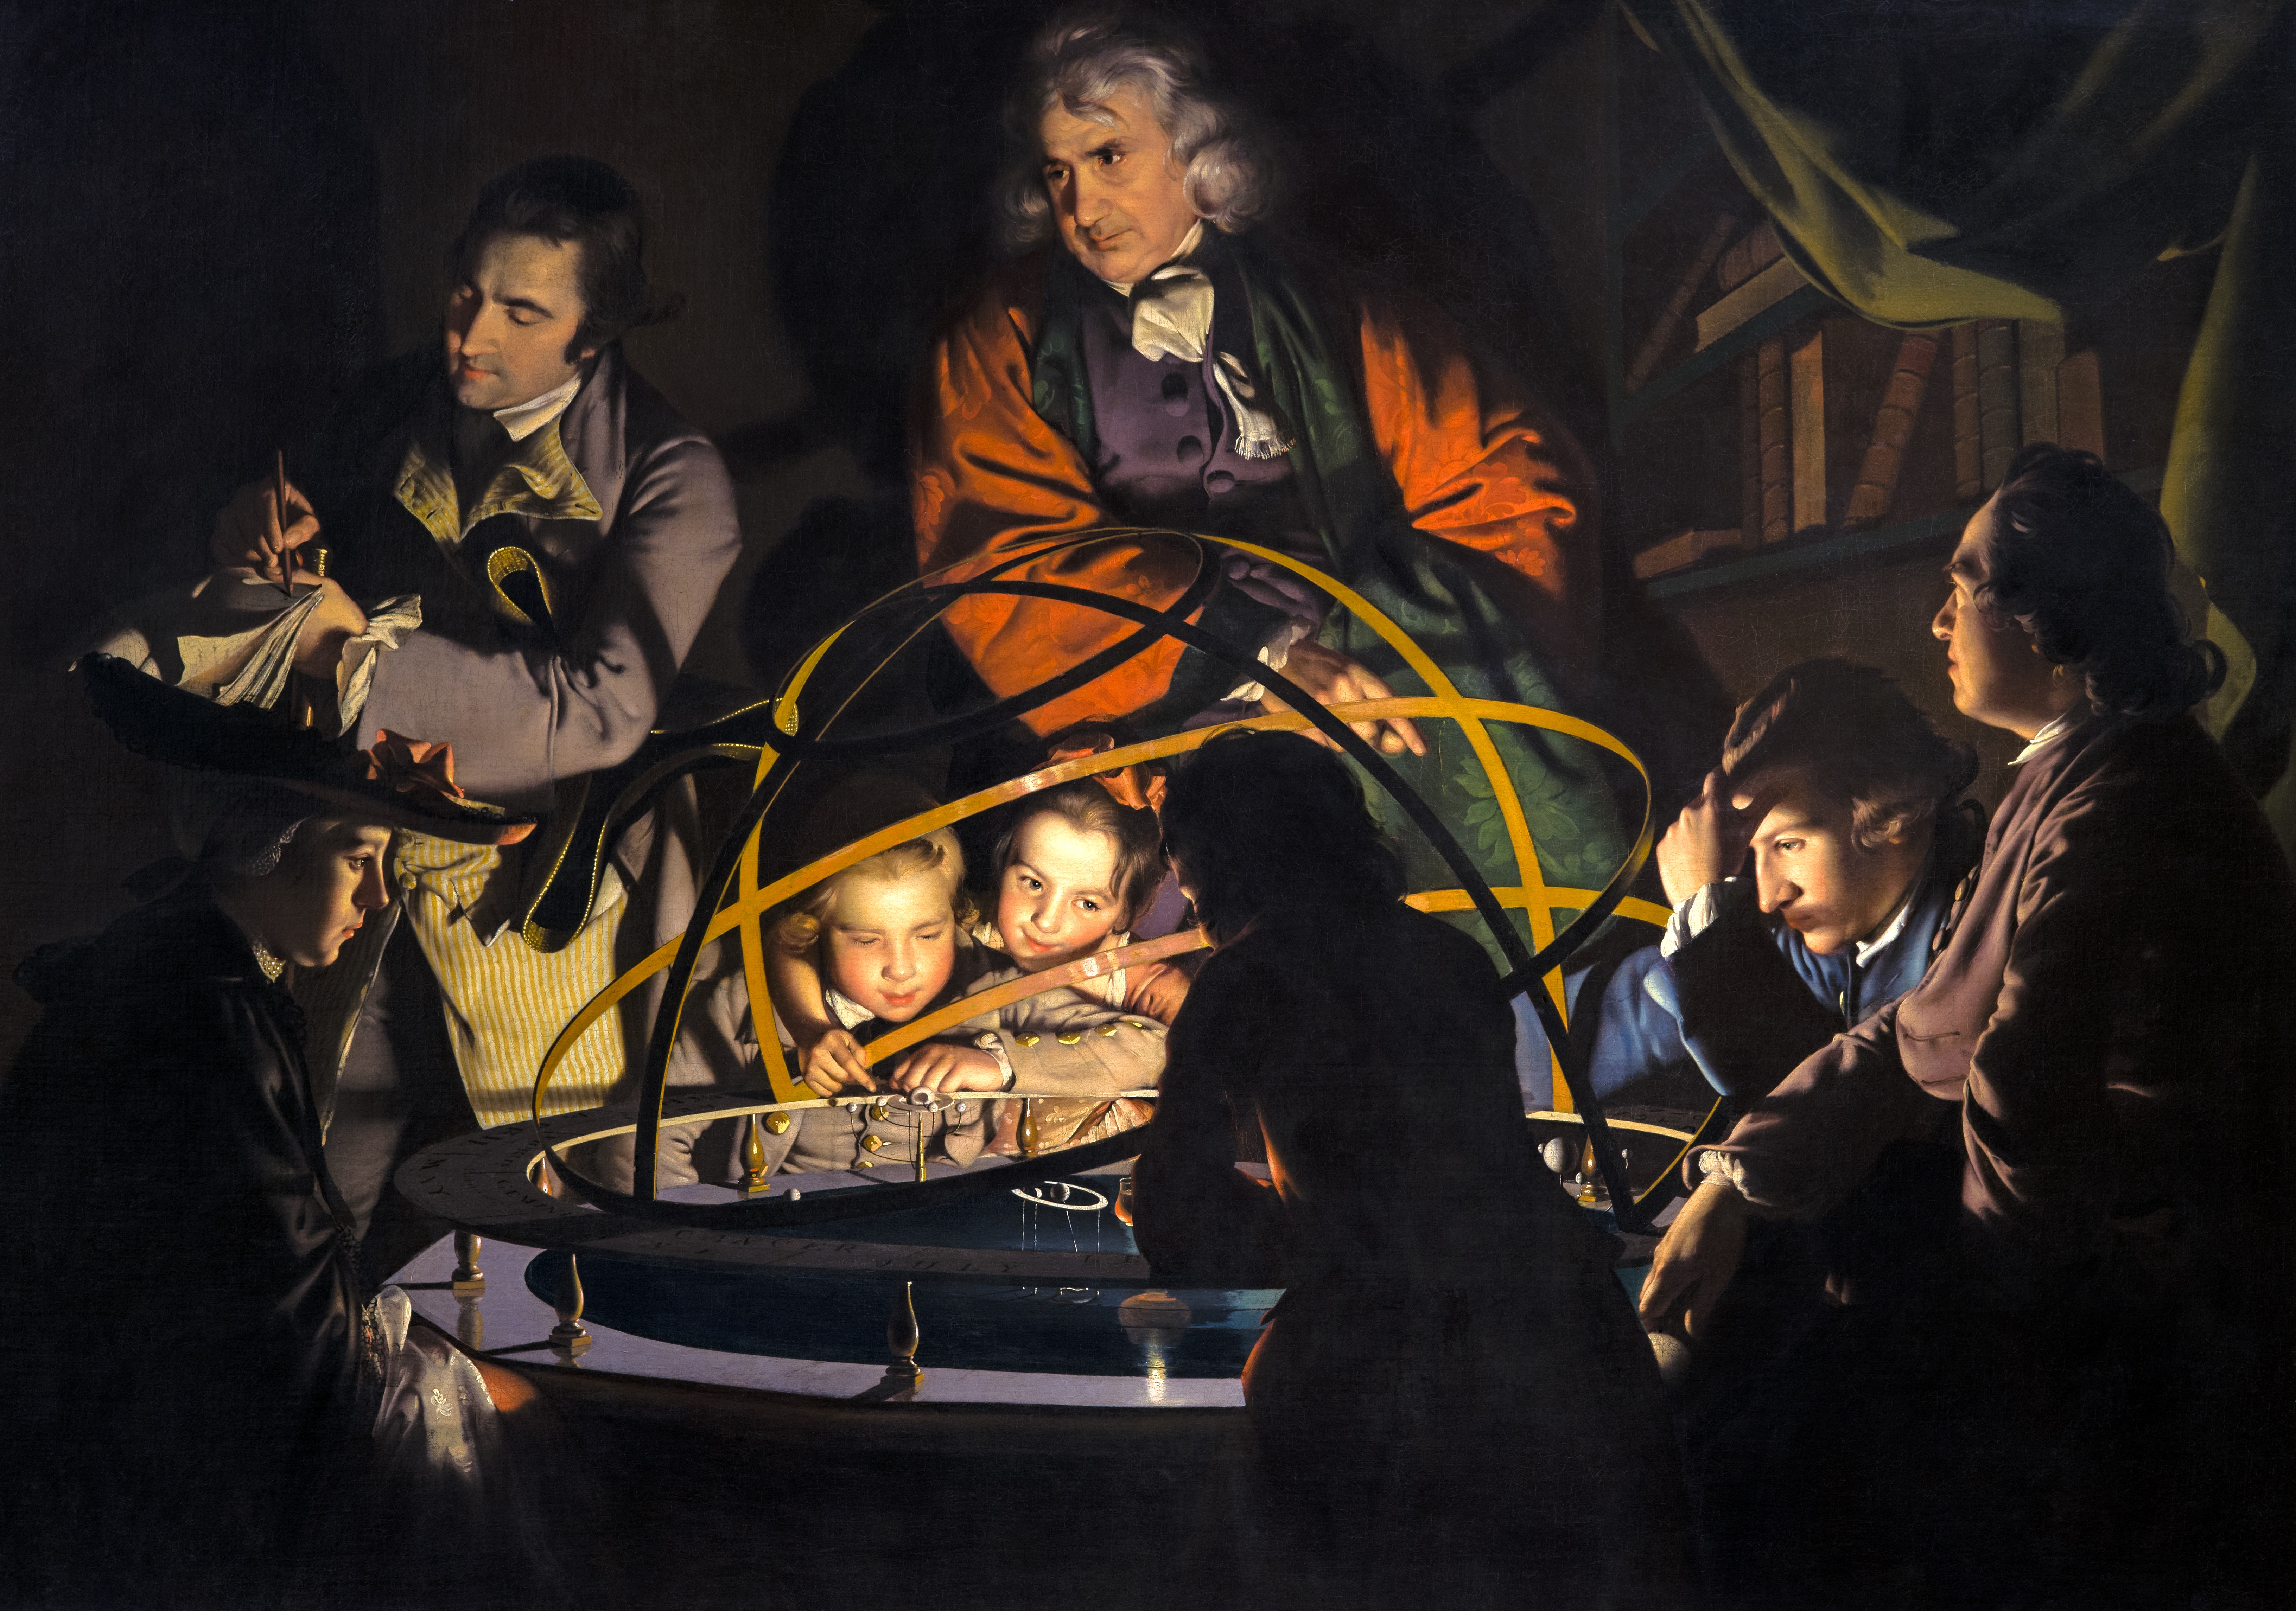
\includegraphics[width=0.9\linewidth]{fig/orrery} 

}

\caption[A scientist and his model]{\textbf{A scientist and his model.} Joseph Wright
of Derby, \emph{A Philosopher Giving a Lecture at the Orrery (in which a
lamp is put in place of the sun)}, c. 1763-65, oil on canvas, Derby
Museums and Art Gallery}\label{fig:orrery}
\end{figure}






\section{What is a model?}\label{what-is-a-model}

\subsection{In your own words}\label{in-your-own-words}

A model is first of all an ambiguous object and a polysemous word. It
therefore seems necessary to start with a semantic study. Among the many
meanings and synonymous proposed by the dictionary, while some definitions are more related to
art, several find echoes in scientific practice. It is sometimes a
question of the physical representation of an object, often on a reduced
scale as in Figure \ref{fig:orrery}, and sometimes of a theoretical
description intended to facilitate the understanding of the way in which
a system works \citep{dictionnarymodel}. It is even sometimes an ideal
to be reached and therefore an ambitious prospect for an introduction.
  
A model is first of all an ambiguous object and a polysemous word. It
therefore seems necessary to start with a semantic study. Among the many
meanings and synonymous proposed by the dictionary, while some definitions are more related to
art, several find echoes in scientific practice. It is sometimes a
question of the physical representation of an object, often on a reduced
scale as in Figure \ref{fig:orrery}, and sometimes of a theoretical
description intended to facilitate the understanding of the way in which
a system works \citep{dictionnarymodel}. It is even sometimes an ideal
to be reached and therefore an ambitious prospect for an introduction.


\bibliography{bib/thesis.bib}

\end{document}
